% The restricted Voronoi tessellation and its Monte-Carlo estimator, in 2D.
%
% NOT SKETCHED. Every cell here is computed as the intersection of the crystal
% outline with the perpendicular-bisector half-plane of each other site,
% clipped by Sutherland-Hodgman; the samples are a real uniform draw in the
% bounding box, split by the same half-space test the code applies and charged
% to the nearest site. The 4/3 quoted in the caption is measured from this
% figure's own geometry, not assumed.
\begin{figure}[!ht]
\centering
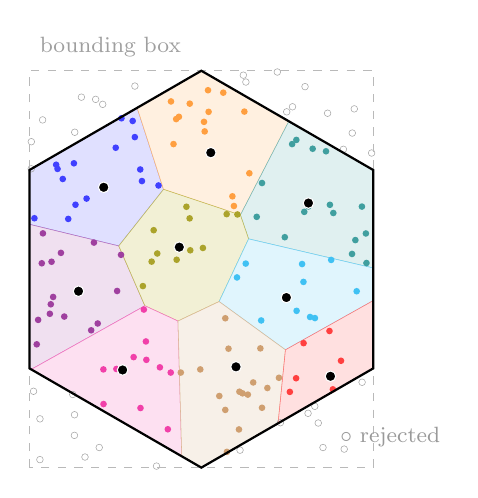
\begin{tikzpicture}[scale=0.80, font=\footnotesize]
  \fill[blue!12] (-1.019,2.562) -- (-2.728,1.575) -- (-2.728,0.712) -- (-1.311,0.369) -- (-0.600,1.267) -- cycle;
  \draw[blue!55, very thin] (-1.019,2.562) -- (-2.728,1.575) -- (-2.728,0.712) -- (-1.311,0.369) -- (-0.600,1.267) -- cycle;
  \fill[orange!12] (1.389,2.348) -- (0.000,3.150) -- (-1.019,2.562) -- (-0.600,1.267) -- (0.620,0.860) -- cycle;
  \draw[orange!55, very thin] (1.389,2.348) -- (0.000,3.150) -- (-1.019,2.562) -- (-0.600,1.267) -- (0.620,0.860) -- cycle;
  \fill[teal!12] (2.728,1.575) -- (1.389,2.348) -- (0.620,0.860) -- (0.750,0.481) -- (2.728,0.019) -- cycle;
  \draw[teal!55, very thin] (2.728,1.575) -- (1.389,2.348) -- (0.620,0.860) -- (0.750,0.481) -- (2.728,0.019) -- cycle;
  \fill[violet!12] (-2.728,0.712) -- (-2.728,-1.575) -- (-2.700,-1.591) -- (-0.896,-0.581) -- (-1.311,0.369) -- cycle;
  \draw[violet!55, very thin] (-2.728,0.712) -- (-2.728,-1.575) -- (-2.700,-1.591) -- (-0.896,-0.581) -- (-1.311,0.369) -- cycle;
  \fill[olive!12] (-0.600,1.267) -- (-1.311,0.369) -- (-0.896,-0.581) -- (-0.371,-0.823) -- (0.282,-0.514) -- (0.750,0.481) -- (0.620,0.860) -- cycle;
  \draw[olive!55, very thin] (-0.600,1.267) -- (-1.311,0.369) -- (-0.896,-0.581) -- (-0.371,-0.823) -- (0.282,-0.514) -- (0.750,0.481) -- (0.620,0.860) -- cycle;
  \fill[cyan!12] (2.728,-0.499) -- (2.728,0.019) -- (0.750,0.481) -- (0.282,-0.514) -- (1.335,-1.280) -- cycle;
  \draw[cyan!55, very thin] (2.728,-0.499) -- (2.728,0.019) -- (0.750,0.481) -- (0.282,-0.514) -- (1.335,-1.280) -- cycle;
  \fill[magenta!12] (-2.700,-1.591) -- (-0.311,-2.970) -- (-0.371,-0.823) -- (-0.896,-0.581) -- cycle;
  \draw[magenta!55, very thin] (-2.700,-1.591) -- (-0.311,-2.970) -- (-0.371,-0.823) -- (-0.896,-0.581) -- cycle;
  \fill[brown!12] (-0.311,-2.970) -- (-0.000,-3.150) -- (1.218,-2.447) -- (1.335,-1.280) -- (0.282,-0.514) -- (-0.371,-0.823) -- cycle;
  \draw[brown!55, very thin] (-0.311,-2.970) -- (-0.000,-3.150) -- (1.218,-2.447) -- (1.335,-1.280) -- (0.282,-0.514) -- (-0.371,-0.823) -- cycle;
  \fill[red!12] (1.218,-2.447) -- (2.728,-1.575) -- (2.728,-0.499) -- (1.335,-1.280) -- cycle;
  \draw[red!55, very thin] (1.218,-2.447) -- (2.728,-1.575) -- (2.728,-0.499) -- (1.335,-1.280) -- cycle;
  % rejected: drawn in the bounding box but outside the crystal
  \draw[gray!70, very thin] (-2.699,2.024) circle (1.5pt);
  \draw[gray!70, very thin] (2.703,1.844) circle (1.5pt);
  \draw[gray!70, very thin] (0.667,3.080) circle (1.5pt);
  \draw[gray!70, very thin] (0.614,-2.873) circle (1.5pt);
  \draw[gray!70, very thin] (-2.664,-1.938) circle (1.5pt);
  \draw[gray!70, very thin] (-0.712,-3.126) circle (1.5pt);
  \draw[gray!70, very thin] (1.801,-2.177) circle (1.5pt);
  \draw[gray!70, very thin] (2.552,-1.795) circle (1.5pt);
  \draw[gray!70, very thin] (-2.010,2.174) circle (1.5pt);
  \draw[gray!70, very thin] (2.428,2.545) circle (1.5pt);
  \draw[gray!70, very thin] (-1.678,2.696) circle (1.5pt);
  \draw[gray!70, very thin] (-2.520,2.370) circle (1.5pt);
  \draw[gray!70, very thin] (-2.562,-2.376) circle (1.5pt);
  \draw[gray!70, very thin] (1.447,2.578) circle (1.5pt);
  \draw[gray!70, very thin] (-1.904,2.731) circle (1.5pt);
  \draw[gray!70, very thin] (-2.700,1.594) circle (1.5pt);
  \draw[gray!70, very thin] (1.694,-2.288) circle (1.5pt);
  \draw[gray!70, very thin] (0.707,2.971) circle (1.5pt);
  \draw[gray!70, very thin] (-1.621,-2.831) circle (1.5pt);
  \draw[gray!70, very thin] (-1.566,2.617) circle (1.5pt);
  \draw[gray!70, very thin] (1.856,-2.442) circle (1.5pt);
  \draw[gray!70, very thin] (-1.055,2.907) circle (1.5pt);
  \draw[gray!70, very thin] (1.255,-2.437) circle (1.5pt);
  \draw[gray!70, very thin] (2.255,1.903) circle (1.5pt);
  \draw[gray!70, very thin] (2.268,-2.856) circle (1.5pt);
  \draw[gray!70, very thin] (-2.563,-3.023) circle (1.5pt);
  \draw[gray!70, very thin] (1.646,2.898) circle (1.5pt);
  \draw[gray!70, very thin] (1.931,-2.831) circle (1.5pt);
  \draw[gray!70, very thin] (2.004,2.476) circle (1.5pt);
  \draw[gray!70, very thin] (-1.847,-2.982) circle (1.5pt);
  \draw[gray!70, very thin] (-2.013,-2.311) circle (1.5pt);
  \draw[gray!70, very thin] (-2.015,-2.638) circle (1.5pt);
  \draw[gray!70, very thin] (1.355,2.498) circle (1.5pt);
  \draw[gray!70, very thin] (-2.042,-1.989) circle (1.5pt);
  \draw[gray!70, very thin] (1.206,3.130) circle (1.5pt);
  \draw[gray!70, very thin] (2.396,2.161) circle (1.5pt);
  % accepted: colored by the node each is charged to
  \fill[orange!75] (0.683,2.502) circle (1.5pt);
  \fill[red!75] (1.504,-1.731) circle (1.5pt);
  \fill[blue!75] (-1.090,2.353) circle (1.5pt);
  \fill[cyan!75] (1.621,-0.202) circle (1.5pt);
  \fill[magenta!75] (-1.075,-1.396) circle (1.5pt);
  \fill[violet!75] (-1.337,-0.346) circle (1.5pt);
  \fill[olive!75] (0.025,0.337) circle (1.5pt);
  \fill[magenta!75] (-1.553,-2.141) circle (1.5pt);
  \fill[violet!75] (-2.533,0.094) circle (1.5pt);
  \fill[orange!75] (-0.184,2.628) circle (1.5pt);
  \fill[cyan!75] (0.705,0.089) circle (1.5pt);
  \fill[brown!75] (-0.017,-1.591) circle (1.5pt);
  \fill[brown!75] (1.048,-1.886) circle (1.5pt);
  \fill[blue!75] (-1.268,2.396) circle (1.5pt);
  \fill[orange!75] (0.053,2.187) circle (1.5pt);
  \fill[orange!75] (0.762,1.523) circle (1.5pt);
  \fill[violet!75] (-2.229,0.259) circle (1.5pt);
  \fill[orange!75] (0.042,2.339) circle (1.5pt);
  \fill[olive!75] (-0.757,0.619) circle (1.5pt);
  \fill[violet!75] (-2.405,-0.708) circle (1.5pt);
  \fill[magenta!75] (-0.966,-2.204) circle (1.5pt);
  \fill[cyan!75] (1.726,-0.759) circle (1.5pt);
  \fill[teal!75] (2.612,0.567) circle (1.5pt);
  \fill[olive!75] (0.573,0.869) circle (1.5pt);
  \fill[brown!75] (0.963,-2.200) circle (1.5pt);
  \fill[brown!75] (-0.326,-1.641) circle (1.5pt);
  \fill[magenta!75] (-0.532,-2.541) circle (1.5pt);
  \fill[brown!75] (0.937,-1.257) circle (1.5pt);
  \fill[teal!75] (2.041,1.022) circle (1.5pt);
  \fill[brown!75] (0.380,-2.234) circle (1.5pt);
  \fill[brown!75] (0.285,-2.013) circle (1.5pt);
  \fill[teal!75] (2.095,0.892) circle (1.5pt);
  \fill[brown!75] (0.380,-0.779) circle (1.5pt);
  \fill[magenta!75] (-0.486,-1.641) circle (1.5pt);
  \fill[olive!75] (-0.176,0.300) circle (1.5pt);
  \fill[blue!75] (-0.970,1.583) circle (1.5pt);
  \fill[violet!75] (-2.591,-0.805) circle (1.5pt);
  \fill[teal!75] (2.549,0.994) circle (1.5pt);
  \fill[olive!75] (-0.392,0.150) circle (1.5pt);
  \fill[red!75] (2.034,-0.981) circle (1.5pt);
  \fill[orange!75] (0.493,1.157) circle (1.5pt);
  \fill[olive!75] (-0.789,0.120) circle (1.5pt);
  \fill[orange!75] (-0.442,1.986) circle (1.5pt);
  \fill[blue!75] (-2.650,0.809) circle (1.5pt);
  \fill[cyan!75] (1.599,0.082) circle (1.5pt);
  \fill[brown!75] (1.232,-1.724) circle (1.5pt);
  \fill[violet!75] (-1.645,-0.862) circle (1.5pt);
  \fill[violet!75] (-1.749,-0.970) circle (1.5pt);
  \fill[teal!75] (2.445,0.462) circle (1.5pt);
  \fill[magenta!75] (-0.873,-1.439) circle (1.5pt);
  \fill[cyan!75] (2.466,-0.350) circle (1.5pt);
  \fill[teal!75] (2.621,0.098) circle (1.5pt);
  \fill[orange!75] (0.115,2.498) circle (1.5pt);
  \fill[teal!75] (1.325,0.508) circle (1.5pt);
  \fill[orange!75] (-0.400,2.383) circle (1.5pt);
  \fill[orange!75] (-0.482,2.663) circle (1.5pt);
  \fill[violet!75] (-2.353,-0.441) circle (1.5pt);
  \fill[orange!75] (0.106,2.841) circle (1.5pt);
  \fill[blue!75] (-1.359,1.928) circle (1.5pt);
  \fill[teal!75] (0.963,1.368) circle (1.5pt);
  \fill[magenta!75] (-0.913,-0.641) circle (1.5pt);
  \fill[cyan!75] (0.566,-0.131) circle (1.5pt);
  \fill[orange!75] (0.517,1.003) circle (1.5pt);
  \fill[olive!75] (-0.186,0.807) circle (1.5pt);
  \fill[brown!75] (0.738,-1.991) circle (1.5pt);
  \fill[violet!75] (-2.390,-0.557) circle (1.5pt);
  \fill[teal!75] (1.441,1.986) circle (1.5pt);
  \fill[cyan!75] (2.061,0.147) circle (1.5pt);
  \fill[magenta!75] (-1.349,-1.584) circle (1.5pt);
  \fill[violet!75] (-1.705,0.422) circle (1.5pt);
  \fill[violet!75] (-2.515,0.569) circle (1.5pt);
  \fill[blue!75] (-1.822,1.121) circle (1.5pt);
  \fill[violet!75] (-2.613,-1.193) circle (1.5pt);
  \fill[teal!75] (2.392,0.242) circle (1.5pt);
  \fill[teal!75] (1.700,0.996) circle (1.5pt);
  \fill[brown!75] (0.604,-1.945) circle (1.5pt);
  \fill[brown!75] (0.406,-2.900) circle (1.5pt);
  \fill[magenta!75] (-0.880,-1.147) circle (1.5pt);
  \fill[blue!75] (-2.113,0.798) circle (1.5pt);
  \fill[red!75] (1.623,-1.174) circle (1.5pt);
  \fill[teal!75] (1.979,1.872) circle (1.5pt);
  \fill[blue!75] (-2.023,1.681) circle (1.5pt);
  \fill[red!75] (2.088,-1.907) circle (1.5pt);
  \fill[olive!75] (0.402,0.874) circle (1.5pt);
  \fill[brown!75] (0.597,-2.544) circle (1.5pt);
  \fill[teal!75] (0.879,0.831) circle (1.5pt);
  \fill[teal!75] (1.767,1.912) circle (1.5pt);
  \fill[blue!75] (-0.943,1.399) circle (1.5pt);
  \fill[brown!75] (0.823,-1.798) circle (1.5pt);
  \fill[orange!75] (0.348,2.802) circle (1.5pt);
  \fill[magenta!75] (-0.658,-1.558) circle (1.5pt);
  \fill[olive!75] (-0.237,0.991) circle (1.5pt);
  \fill[violet!75] (-2.176,-0.752) circle (1.5pt);
  \fill[blue!75] (-1.998,1.023) circle (1.5pt);
  \fill[cyan!75] (1.803,-0.776) circle (1.5pt);
  \fill[olive!75] (-0.700,0.249) circle (1.5pt);
  \fill[magenta!75] (-1.555,-1.591) circle (1.5pt);
  \fill[olive!75] (-0.928,-0.268) circle (1.5pt);
  \fill[blue!75] (-2.283,1.592) circle (1.5pt);
  \fill[brown!75] (0.431,-1.262) circle (1.5pt);
  \fill[blue!75] (-2.305,1.658) circle (1.5pt);
  \fill[red!75] (2.217,-1.454) circle (1.5pt);
  \fill[blue!75] (-1.056,2.097) circle (1.5pt);
  \fill[brown!75] (0.654,-1.971) circle (1.5pt);
  \fill[orange!75] (-0.356,2.419) circle (1.5pt);
  \fill[blue!75] (-0.680,1.329) circle (1.5pt);
  \fill[blue!75] (-2.200,1.432) circle (1.5pt);
  \fill[teal!75] (1.508,2.052) circle (1.5pt);
  \fill[cyan!75] (0.950,-0.814) circle (1.5pt);
  \fill[violet!75] (-2.378,0.118) circle (1.5pt);
  \fill[red!75] (1.405,-1.948) circle (1.5pt);
  \fill[violet!75] (-1.275,0.228) circle (1.5pt);
  \fill[teal!75] (1.634,0.910) circle (1.5pt);
  \fill[cyan!75] (1.512,-0.661) circle (1.5pt);
  \draw[gray!55, dashed, thin] (-2.728,-3.150) rectangle (2.728,3.150);
  \draw[black, thick] (2.728,1.575) -- (0.000,3.150) -- (-2.728,1.575) -- (-2.728,-1.575) -- (-0.000,-3.150) -- (2.728,-1.575) -- cycle;
  \fill[black] (-1.550,1.300) circle (2.4pt);
  \draw[white, line width=0.4pt] (-1.550,1.300) circle (2.4pt);
  \fill[black] (0.150,1.850) circle (2.4pt);
  \draw[white, line width=0.4pt] (0.150,1.850) circle (2.4pt);
  \fill[black] (1.700,1.050) circle (2.4pt);
  \draw[white, line width=0.4pt] (1.700,1.050) circle (2.4pt);
  \fill[black] (-1.950,-0.350) circle (2.4pt);
  \draw[white, line width=0.4pt] (-1.950,-0.350) circle (2.4pt);
  \fill[black] (-0.350,0.350) circle (2.4pt);
  \draw[white, line width=0.4pt] (-0.350,0.350) circle (2.4pt);
  \fill[black] (1.350,-0.450) circle (2.4pt);
  \draw[white, line width=0.4pt] (1.350,-0.450) circle (2.4pt);
  \fill[black] (-1.250,-1.600) circle (2.4pt);
  \draw[white, line width=0.4pt] (-1.250,-1.600) circle (2.4pt);
  \fill[black] (0.550,-1.550) circle (2.4pt);
  \draw[white, line width=0.4pt] (0.550,-1.550) circle (2.4pt);
  \fill[black] (2.050,-1.700) circle (2.4pt);
  \draw[white, line width=0.4pt] (2.050,-1.700) circle (2.4pt);
  \node[gray!75, anchor=south west, font=\footnotesize]
    at (-2.72,3.22) {bounding box};
  \node[anchor=north west, font=\footnotesize] at (2.05,-2.35)
    {\textcolor{gray!80}{$\circ$ rejected}};
\end{tikzpicture}
\caption{The restricted Voronoi tessellation and the Monte-Carlo estimator of
the nodal volumes, drawn in two dimensions. Black discs are cluster-dynamics
nodes; the shaded polygons are their Voronoi cells, each the set of points
nearer that node than any other, clipped to the crystal. Samples are drawn
uniformly in the dashed bounding box: those failing the half-space test
$\bm N\xv\le\bm b$ are rejected (open circles) and the survivors are charged to
their nearest node (filled, colored by cell), giving
$V_j=(M_j/M)\,V_\Omega$. \emph{Restricted} is the whole point --- a sample in a
corner of the box lies outside the crystal and belongs to no node, where an
unrestricted tessellation would charge it to whichever boundary node happened
to be nearest. For this hexagon the box carries $4/3$ of the crystal area, and
the same ratio holds for the prism in three dimensions, so a third of all
samples are discarded by construction.}
\label{fig:voronoi}
\end{figure}
